\documentclass[11pt]{article}
\usepackage{enumitem}
%\setlist[itemize]{nosep}       % no extra separation
%\setlist[enumerate]{nosep}
%\setlist[itemize]{topsep=0pt}	% no top separation
%\setlist[enumerate]{topsep=0pt}

\usepackage[margin=1in]{geometry}
\usepackage{tikz}
\usepackage{mathtools}
\usepackage[final]{pdfpages}
\usepackage[makeroom]{cancel}
\date{}

\begin{document}

\begin{center}
\noindent{\bf {\LARGE COMP 3804/Math 3804: Assignment 2}}\\
\vspace{0.5cm}
\noindent{\bf {\LARGE Ryan Lo (101117765)}}\\
\vspace{0.5cm}
{\bf Due Date: Sunday, October $23^{rd}$ at 11:59PM}
\end{center}
\noindent School of Computer Science\hfill{Carleton University}

\noindent \hrulefill

Your assignment should be submitted online on Brightspace as a single .pdf file.  The filename should contain your name and student number. No late assignments will be accepted.You can type your assignment or you can upload a scanned copy of it.  Please, use a good image capturing device. Make sure that your upload is clearly readable. If it is difficult to read, it will not be graded.

%%%%%%%%%%%% NEW SECTION %%%%%%%%%%%%%%%%%
\section*{Question 1 [15 marks]}
Consider a $4-heap$ to be a heap-ordered tree in which each internal node has 4 children, all leaves are on at most two adjacent levels, and, on the last level, all
leaves are as much to the left as possible. Let $n$ be the total number of nodes in the tree and  assume that $n=4*k + 1 $, for some positive integer $k$.

 \begin{enumerate}
\item State precisely:
 	\begin{itemize}
 		\item
 		how many leaf-nodes a $4-heap$ on $n$ nodes can have minimally and maximally,

		For $k = 1$, $n=4*1 + 1 = 5$, the min and max leaf nodes would be 4.

		For $k = 2$, $n=4*2 + 1 = 9$, the min and max leaf nodes would be 7.

		For $k = 3$, $n=4*3 + 1 = 13$, the min and max leaf nodes would be 10.

		For $k = 4$, $n=4*4 + 1 = 17$, the min and max leaf nodes would be 13.

		Looking at this pattern we can see that the number of min and max leaf nodes are $n-k$.

		A $4-heap$ on $n$ nodes can have minimally and maximally $n-k$ leaf nodes.

 		\item 
 		how many nodes there are on each level, i,  (excluding the lowest level),

		$i = 1$, $n = 1$

		$i = 2$, $n = 4$

		$i = 3$, $n = 16$

		$i = 4$, $n = 64$

		On each level, i, there are $4^{i-1}$ nodes on that level.

 		\item   an expression, phrased in terms of $n$, for the height of the tree,
 		
		The height of the tree $= floor(log_4 (n*(4-1))) + 1$

 		\item
 		how many nodes there are on all levels  together (excluding the lowest level),

		Sum up all the nodes from each level.

		$\sum_{n=1}^{i} 4^{n-1}$

 		\item
 		a relation between  the total number of internal nodes and the number of leaves.

		$k = n - leaves$
 		
 	\end{itemize}

	\item Assume the tree is stored in an array H[1 ... n]. (Note: we start with index 1 not 0.) Give address formulae for: the children of an internal node stored at H[i] and the parent node of a node stored at H[i].
	
	The children of the node H[i] is: ceiling $4*i+1-n$, where $n \in ({0,1,2,3})$

	The parent of the node H[i] is: ceiling $(i-1)/4$
	
\end{enumerate}

%%%%%%%%%%%% NEW SECTION %%%%%%%%%%%%%%%%%
\section*{Question 2 [11 marks]}

\begin{enumerate}
	\item  For standard  binary heaps, we also store the heap in an array H[1....n]. Now,  state parent/child index relations, but use the bit representation of the array indices.  So, state (child to parent) and (parent to child) array index relations using the binary representation of indices. So,  
	      we get e.g., the children of the root are stored at binary(10) and binary(11) and the parent of binary(10) and binary(11) is the root stored at binary(1).
	
	Looking at the parent/child relations and it's bit representation, removing the last bit of the child node gives you the parent node.

	\item Let the $i^{th}$parent(node) be recursively defined as follows:
	
	\ \ \ \ \ \ \ \ \ \  for $i=0$ the $i^{th}$parent(node) is the node itself.
	
\ \ \ \ \ \ \ \ \ \  for $i>1$, $i^{th}$parent(node) is the parent of  $(i-1)^{st}$parent(node).		

		Now, state a simple formula (in binary) for the $i^{th}$ parent of a node stored at binary$(b_1 ... b_m)$.

		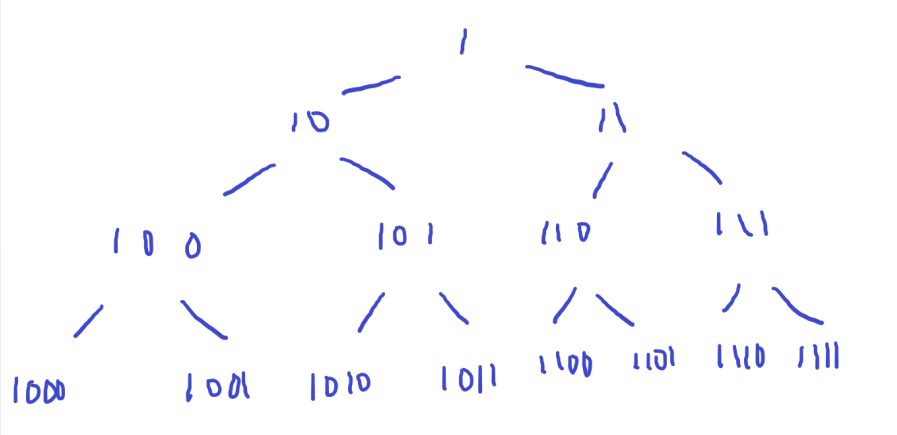
\includegraphics[width=\textwidth]{q2.png}

		As you can see from this picture, as you go up the tree, from the 4th parent node to the 2nd parent node it would be a right bit shift of 2.
		Let $i$ be the $i^{th}$ parent of a node, let $j$ be the $(i-1)^{st}$parent(node), then the simple formula is as follows:
		$i^{th}$ parent of a node $=$ $j >> (j-i)$. The node is right shifted the difference between the two nodes.

\end{enumerate}

%
\section*{Question 3 [20 marks]}
Suppose that we want to find a minimum spanning tree of the graph shown on Figure~\ref{fig:MSTgraph}.
\begin{itemize}
	\item Run Prim's algorithm on this graph. Start from vertex $A$ and whenever there is a choice of vertices, always select in the alphabetic order. Draw a table showing the intermediate values at each step.
	
	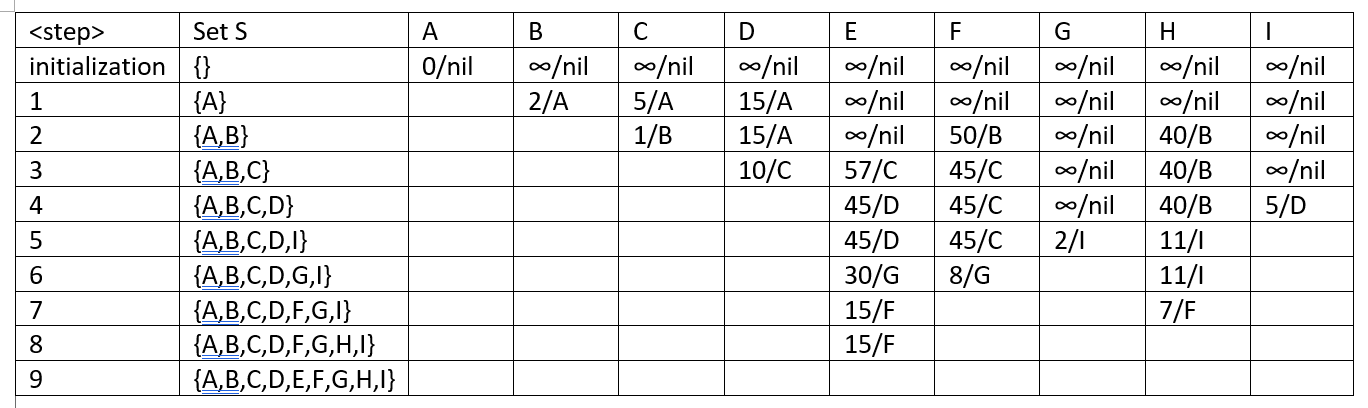
\includegraphics[width=\textwidth]{PRIV.png}
	
	\item Run Kruskal's algorithm on the same graph. Clearly show the disjoint-set data structure (i.e., the structure of the directed trees) at every intermediate step, assuming union using path compression.
	
	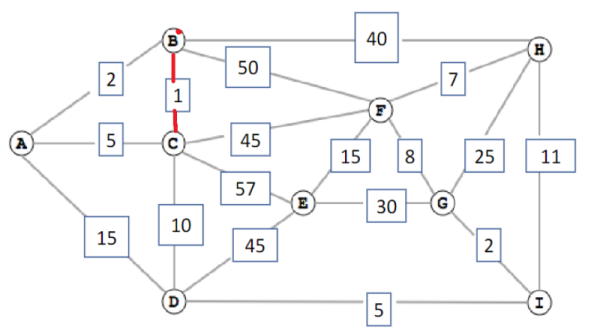
\includegraphics[width=\textwidth]{1.png}

	Edges: $\cancel{1},2,2,5,5,7,8,10,11,15,15,25,30,40,45,45,50,57$

	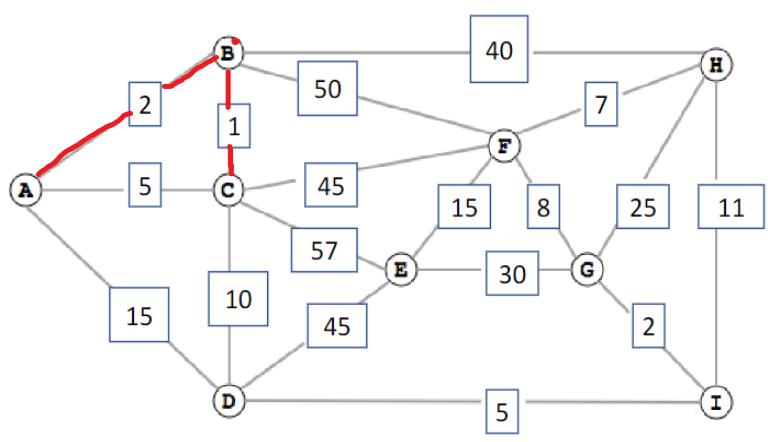
\includegraphics[width=\textwidth]{2.png}

	Edges: $\cancel{1,2},2,5,5,7,8,10,11,15,15,25,30,40,45,45,50,57$

	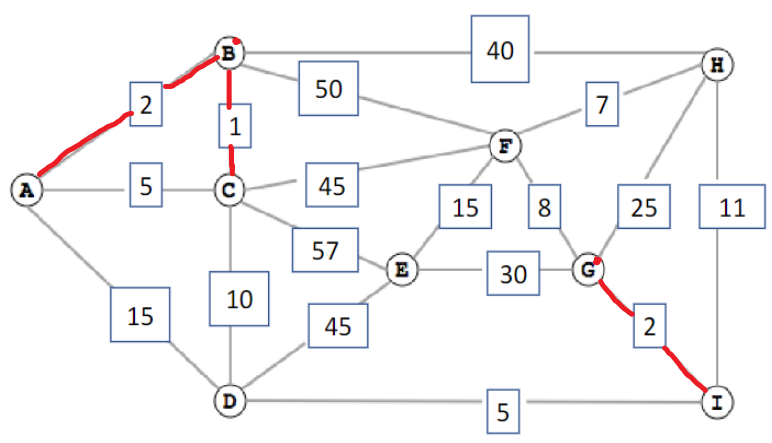
\includegraphics[width=\textwidth]{3.png}

	Edges: $\cancel{1,2,2},5,5,7,8,10,11,15,15,25,30,40,45,45,50,57$

	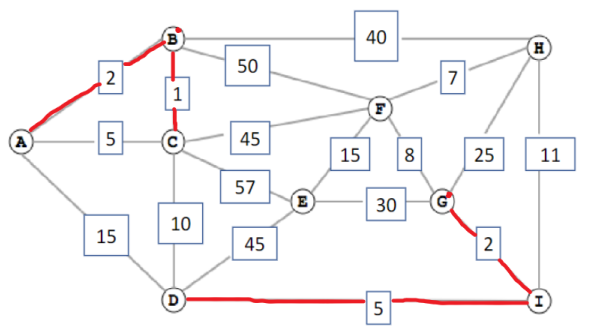
\includegraphics[width=\textwidth]{4.png}

	Edges: $\cancel{1,2,2,5,5},7,8,10,11,15,15,25,30,40,45,45,50,57$

	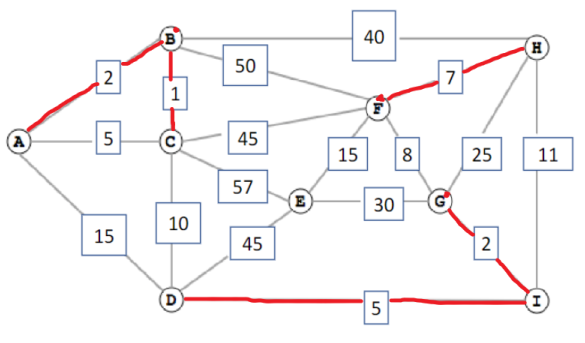
\includegraphics[width=\textwidth]{5.png}

	Edges: $\cancel{1,2,2,5,5,7},8,10,11,15,15,25,30,40,45,45,50,57$

	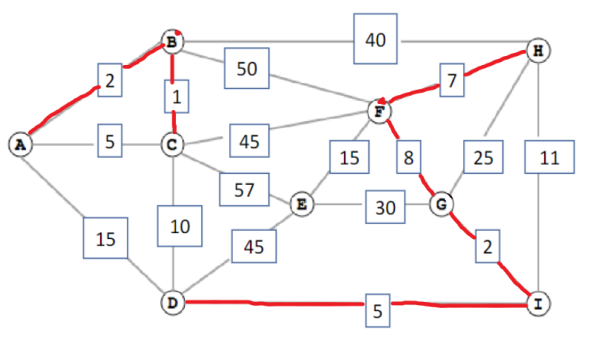
\includegraphics[width=\textwidth]{6.png}

	Edges: $\cancel{1,2,2,5,5,7,8},10,11,15,15,25,30,40,45,45,50,57$

	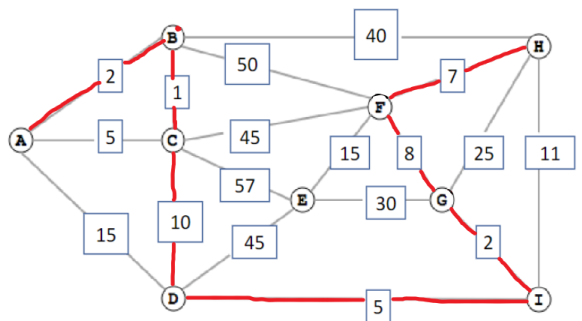
\includegraphics[width=\textwidth]{7.png}

	Edges: $\cancel{1,2,2,5,5,7,8,10},11,15,15,25,30,40,45,45,50,57$

	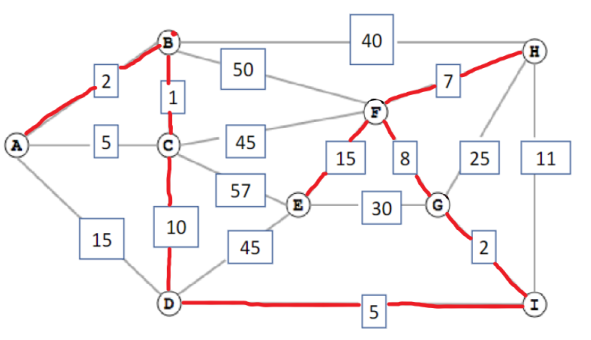
\includegraphics[width=\textwidth]{8.png}

	Edges: $\cancel{1,2,2,5,5,7,8,10,11,15,15,25,30,40,45,45,50,57}$

\end{itemize}

\begin{figure}[t]
	\centerline{\resizebox{!}{0.8\textwidth}{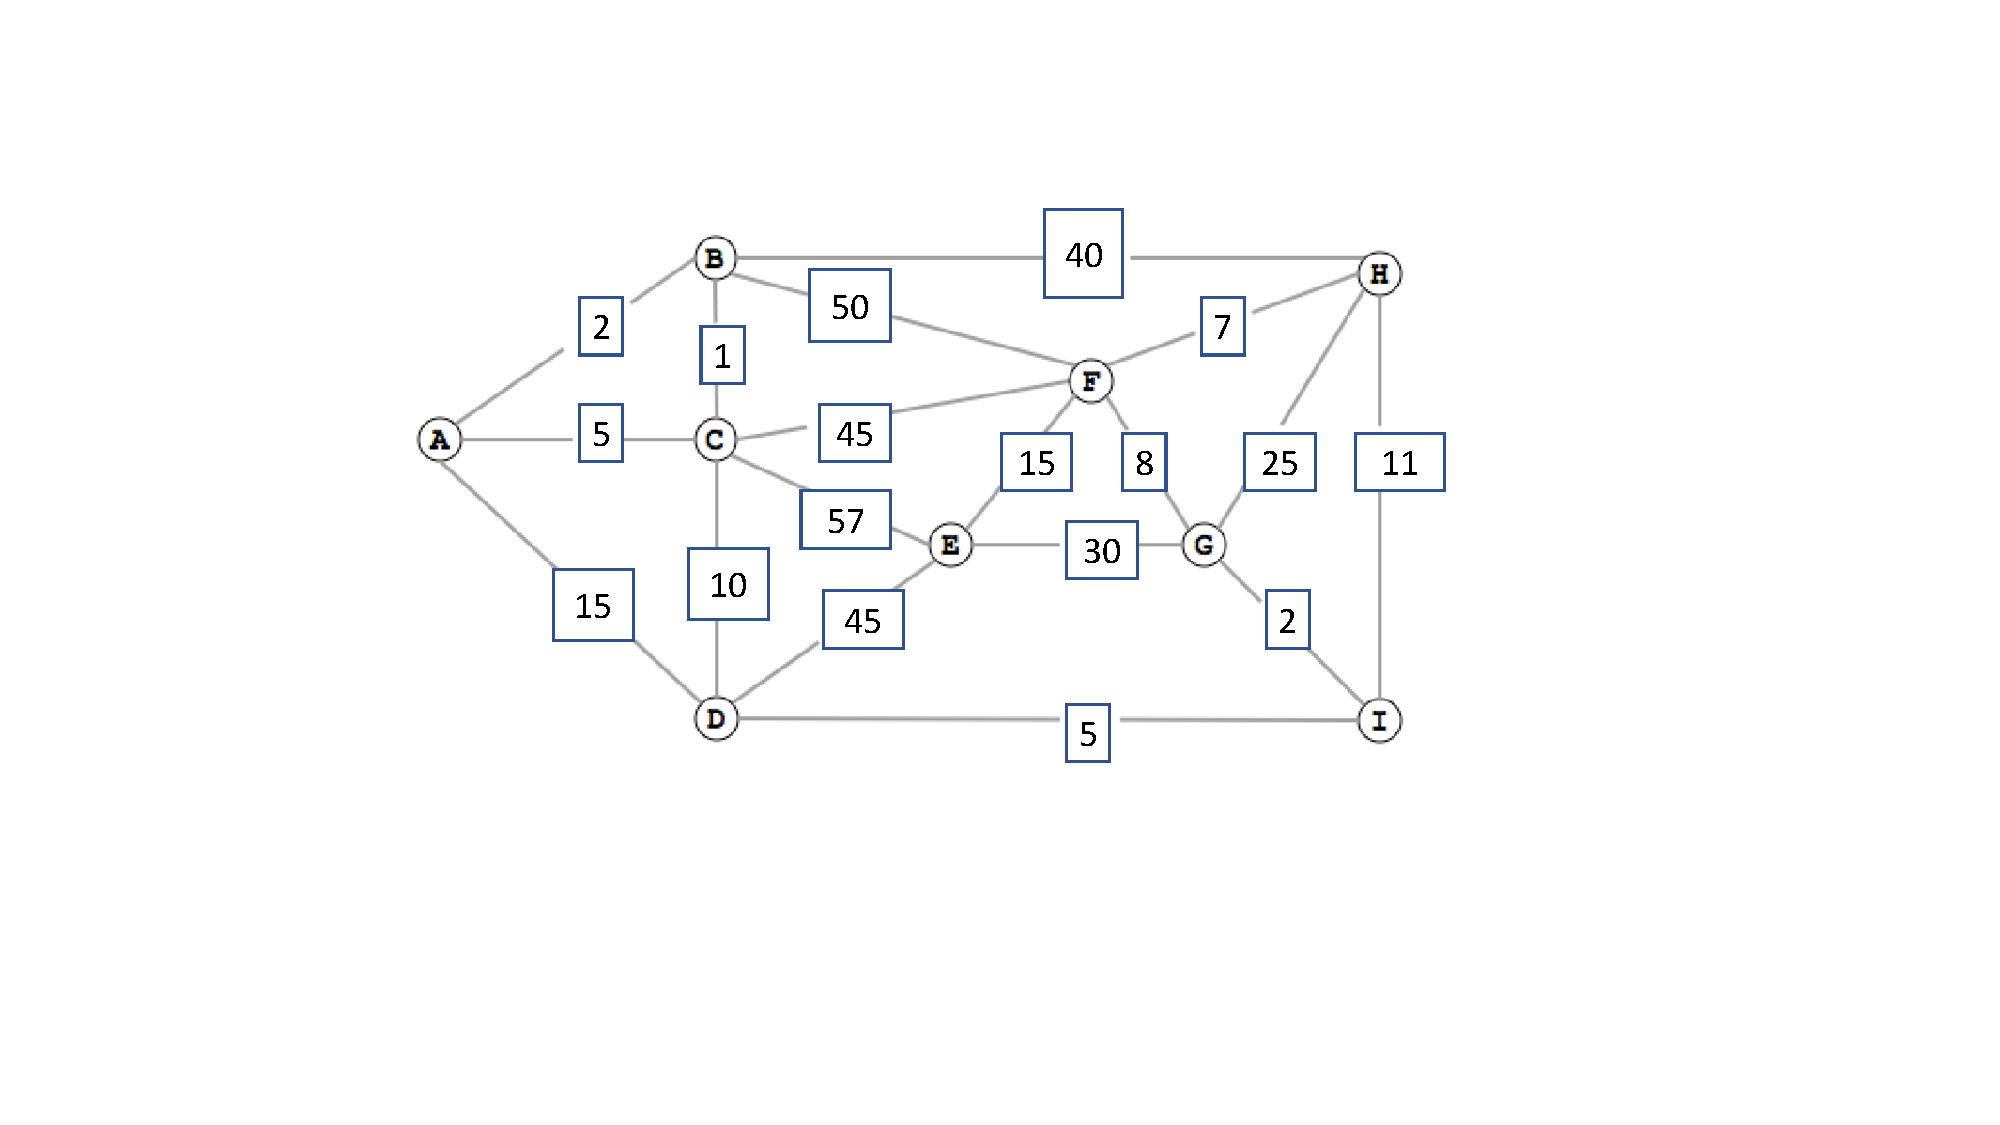
\includegraphics{mst.pdf}}}
	\caption{The input graph for Question 3.}
	\label{fig:MSTgraph}
\end{figure}

%%%%%%%%%%%% NEW SECTION %%%%%%%%%%%%%%%%%
\section*{Question 4 [20 marks]}
 Let $G= (V,E)$ be a graph with distinct weights.
 Let $e_{i}, i=1...|E|$ be the list of edges, sorted by weight. Let $j < k$, be two indices such that $e_j$ is not in the minimum spanning tree of G, but $e_k$ is. Prove or disprove that  the  

 We are given that $e_j$ is not in the minimum spanning tree of G. 
 The definition of minimum spanning tree is as follows "a subset of the edges of a connected, edge-weighted undirected graph that connects all the vertices together, without any cycles and with the minimum possible total edge weight".
 Since $e_j$ is not in the minimum spanning tree of G, if we were to remove $e_j$ from G, the graph of G will still be connected as per defintion of minimum spanning tree because a mimimum spanning tree must still exist when we remove $e_j$.
 Therefore, the removal of $e_{j}$ (from the graph) cannot disconnect $G$.


%\begin{center}
%\noindent{\bf End of Assignment 1.}
%\end{center}

\end{document}